\section{Identification du sens du résultat}
\subsection{Restriction et motivations}
\begin{frame}{Restriction et motivation}
\begin{itemize}
	\item Uniquement les décisions à une demande de la catégorie considérée
	\begin{itemize}
		\item Raison: plus de $50\%$ des documents dans la majorité des catégories
	\end{itemize}
	\item Classification binaire
	\begin{itemize}
		\item Raison: le sens d'un résultat est pratiquement toujs une de ces deux valeurs : \textbf{accepte} ou \textbf{rejette}
	\end{itemize}
\end{itemize}
\begin{figure}
	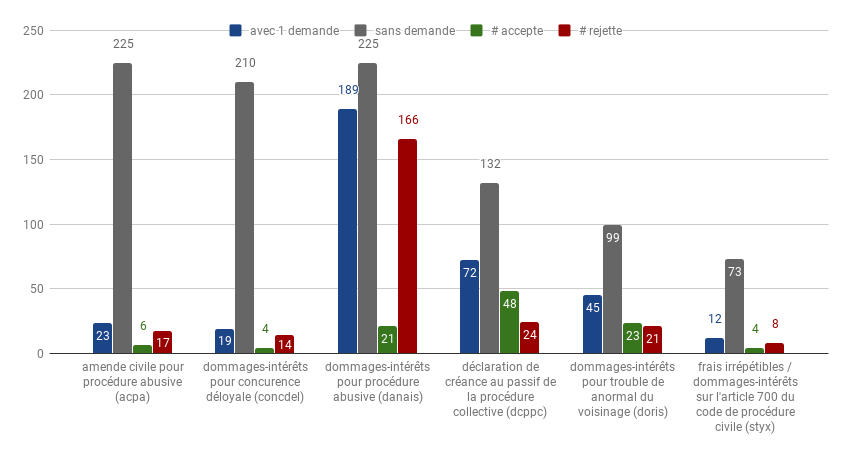
\includegraphics[width=0.8\textwidth]{chartDataset1dmd.png}
	%\caption{\scriptsize Répartitions des sens de résultats (cas à une demande de la catégorie).}
\end{figure}
\end{frame}

%\subsection{Formulation et décomposition du problème}
%\begin{frame}{}
%
%\end{frame}
\subsection{Synthèse bibliographique}
% t^ache semblable, méthodes récentes, pquoi ce n'est pas applicable à notre cas?
% Justification d'une méthode propre aux données qu'on a

\begin{frame}{NBSVM \cite{wang2012nbsvm}}
$x^{(k)} = f^{(k)}$ vecteur intitial des caractéristiques du texte $k$

$r = \log \left( \frac{p/\vert\vert p \vert\vert_1}{q / \vert\vert q \vert\vert_1}\right)$, vecteur poids du classifieur bayésien multinomial

avec $p=\alpha + \sum_{i:y^{(i)}=1f^{(i)}}$, $q=\alpha + \sum_{i:y^{(i)}=-1f^{(i)}}$

L'idée: transformer les caractéristiques réduites à leur simple présence $\widehat{f}^{(k)}$ avec $r$ ($\overset{\sim}{f}^{(k)} = \widehat{r} \circ \widehat{f}^{(k)}$)

$\widehat{r}$ est calculé avec $\widehat{f}^{(k)}$

les nouveaux $x^{(k)} = \overset{\sim}{f}^{(k)}$ sont utilisés dans un SVM.

\end{frame}

\begin{frame}{fastText \cite{grave2017fasttextcls}}
\begin{figure}
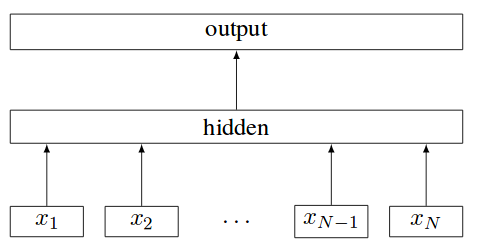
\includegraphics[width=0.5\textwidth]{fastTextArchi.png}
\caption{\scriptsize Architecture similaire au model CBOW : le label remplace le mot au milieu.}
\end{figure}

Entrainement : $min \left(-\frac{1}{N}y_n \cdot \sum\limits_{n=1}^N y_n \cdot \log{f(B\cdot A\cdot x_n)}\right)$ 

où $f$ est la fonction softmax $f(z) = \left[ \frac{e^{z_j}}{\sum\limits_{k=1}^K e^{z_k}} \right]_{\forall j \in \lbrace 1, ..., K \rbrace} $
\end{frame}

\begin{frame}{Résultats obtenus avec fastText et NBSVM}
\textbf{Influence du déséquilibre et de la (très) faible taille des données}
\begin{table}
\scriptsize
\begin{tabular}{|l|l|l|l|l|l|l|l|l|}
\hline
\textbf{Cat. Dmd.} & \textbf{Algo.} & \textbf{Préc.}   & \textbf{Préc. équi.} & \textbf{err-0} & \textbf{err-1} & \textbf{f1-0}  & \textbf{f1-1}  & \textbf{f1-macro-avg} \\ \hline
\textbf{dcppc}       & nbsvm      & 0.875 & 0.812        & 0.375 & 0     & 0.752 & 0.916 & \textbf{0.834}        \\ \hline
danais      & fasttext   & \textbf{0.888} & 0.5          & 1     & 0     & 0     & 0.941 & 0.47         \\ \hline
danais      & nbsvm      & 0.888 & 0.5          & 0     & 1     & 0.941 & 0     & 0.47         \\ \hline
concdel     & fasttext   & 0.775 & 0.5          & 1     & 0     & 0     & 0.873 & 0.437        \\ \hline
concdel     & nbsvm      & 0.775 & 0.5          & 0     & 1     & 0.873 & 0     & 0.437        \\ \hline
acpa        & fasttext   & 0.745 & 0.5          & 1     & 0     & 0     & 0.853 & 0.426        \\ \hline
acpa        & nbsvm      & 0.745 & 0.5          & 0     & 1     & 0.853 & 0     & 0.426        \\ \hline
doris       & nbsvm      & 0.5   & 0.492        & 0.85  & 0.167 & 0.174 & 0.63  & 0.402        \\ \hline
dcppc       & fasttext   & 0.667 & 0.5          & 0     & 1     & 0.8   & 0     & 0.4          \\ \hline
styx        & fasttext   & 0.667 & 0.5          & 1     & 0     & 0     & 0.8   & 0.4          \\ \hline
styx        & nbsvm      & 0.667 & 0.5          & 0     & 1     & 0.8   & 0     & 0.4          \\ \hline
doris       & fasttext   & 0.523 & 0.5          & 0     & 1     & 0.686 & 0     & 0.343        \\ \hline
\end{tabular}

\end{table}
0 == accepte

1 == rejette

\end{frame}

%\begin{frame}{Extension de la Régression PLS: Gini-PLS}
%Combinaison du Gini et du PLS1 (unilabel) \cite{souissi2013gini}:
%\begin{enumerate}
%\setlength\itemsep{1.5em}
%\item PLS (Régression partielle des moindres carrés): réduction supervisée des dimensions $x_1, x_2, ..., x_p$ en composantes orthogonales $t_1, ...., t_h$
%
%$t_h = w_{h1} x_1 + \cdots + w_{hj} x_j + \cdots + w_{hp} x_p$
%
%avec $w_{hj} = \frac{cov(u_{(h-1)j}, \epsilon_h)}{\sqrt{\sum_p^{j=1} cov^2(u_{(h-1)j}, \epsilon_h)}}$
%, $y=c_1 t_1 + ... + c_h t_h + \epsilon_h$,
%
%et $x_j=\beta_{1j} t_1 + ... + \beta_{hj} t_h + u_{(h-1)j}$
%
%\item Gini: élimination de la sensibilité au \textit{outliers} en remplaçant la covariance $cov(x_j, y)$ par la covariance de Gini $cog(y; x_j) := cov(y; R(x_j))$
%\end{enumerate}
%
%\end{frame}

\begin{frame}{Application des extensions de la Régression PLS (1)}
PLS standard (Régression partielle des moindres carrés) 

Réduction supervisée des dimensions $x_1, x_2, ..., x_p$ en composantes orthogonales $t_1, ...., t_h$

$t_h = w_{h1} x_1 + \cdots + w_{hj} x_j + \cdots + w_{hp} x_p$

avec $w_{hj} = \frac{cov(u_{(h-1)j}, \epsilon_h)}{\sqrt{\sum_p^{j=1} cov^2(u_{(h-1)j}, \epsilon_h)}}$
, $y=c_1 t_1 + ... + c_h t_h + \epsilon_h$,

et $x_j=\beta_{1j} t_1 + ... + \beta_{hj} t_h + u_{(h-1)j}$


\end{frame}

\begin{frame}{Application des extensions de la Régression PLS (2)}

\begin{enumerate}
\setlength\itemsep{1.5em}

\item Gini-PLS: 
élimination de la sensibilité au \textit{outliers} en remplaçant la covariance $cov(x_j, y)$ par la covariance de Gini $cog(y; x_j) := cov(y; R(x_j))$ pour l'estimation des résidus $u_{(h)j}$ et des poids $w_{hj}$ \cite{mussard2018ginipls}

\item Logit-PLS:  $\forall j > 1$, les $w_{hj} $ sont les coefficients de la régression logistique de $y$ sur les composantes $t_1, ..., t_{h-1}, u_{(h-1)j}$ \cite{tenenhaus2005logitpls}

\item Gini-Logit-PLS: covariance Gini pour $u_{(h)j}$ et coefficient Logit pour les $w_{hj}$
\end{enumerate}
\end{frame}


\begin{frame}{Résultats: meilleures configurations}
\begin{table}[]
\tiny
\label{my-label}
\begin{tabular}{|l|l|l|l|l|l|l|l|l|l|}
\hline
\textbf{Vecteur} & \textbf{classifieur} & \textbf{F1} & \textbf{min} & \textbf{Cat. min} & \textbf{max} & \textbf{Cat. max} & \textbf{F1 - 1$^{er}$F1} & \textbf{max - min} & \textbf{rang} \\ \hline
GSS*TF                 & Tree                & \textbf{0.668}     & 0.5                 & doris                  & 0.92               & dcppc                 & \textbf{0}                    & \textbf{0.42}           & 1             \\ \hline
AVG-G*TF      & LogitPLS         & \textbf{0.648}     & 0.518               & danais                 & 0.781              & dcppc                 & \textbf{0.02}                 & \textbf{0.263}          & 13            \\ \hline
AVG-G*TF      & StandardPLS      & \textbf{0.636}     & 0.49                & danais                 & 0.836              & dcppc                 & \textbf{0.032}                & \textbf{0.346}          & 24            \\ \hline
DELTADF*TF             & GiniPLS          & \textbf{0.586}     & 0.411               & danais                 & 0.837              & dcppc                 & \textbf{0.082}                & \textbf{0.426}          & 169           \\ \hline
DELTADF*TF             & GiniLogitPLS     & \textbf{0.578}     & 0.225               & styx                   & 0.772              & dcppc                 & \textbf{0.09}                 & \textbf{0.547}          & 220           \\ \hline
\end{tabular}
AVG-G == Moyenne des métriques globales de pondération
\end{table}
\scriptsize

En moyenne, la meilleure zone est la partie principale (litige\_motifs\_dispositif)

Les extensions du PLS ne sont pas très éloignées (si on choisi le bon shéma de vectorisation)

\end{frame}

\begin{frame}{Résultats pour chaque classe}
\begin{table}[]
\tiny
\centering
\label{my-label}
\begin{tabular}{|l|l|l|l|l|}
\hline
\textbf{Cat. Dmd} & \textbf{zone}                                    & \textbf{Vecteur}      & \textbf{classifieur} & \textbf{F1}    \\ \hline
\textbf{acpa}     & \textbf{demande\_resultat\_a\_resultat\_context} & \textbf{DBIDF*TF}           & \textbf{Tree}        & \textbf{0.846} \\ \hline
acpa              & litige\_motifs\_dispositif                       & DELTADF*TF                  & StandardPLS       & 0.697          \\ \hline
acpa              & litige\_motifs\_dispositif                       & AVERAGEGlobals*TF           & LogitPLS          & 0.683          \\ \hline
\textbf{concdel}  & \textbf{litige\_motifs\_dispositif}              & \textbf{GSS*TF}             & \textbf{Tree}        & \textbf{0.798} \\ \hline
concdel           & motifs                                           & IDF*TF                      & GiniLogitPLS      & 0.703          \\ \hline
concdel           & context                                          & DBIDF*LOGAVE                & StandardPLS       & 0.657          \\ \hline
\textbf{danais}   & \textbf{demande\_resultat\_a\_resultat\_context} & \textbf{CHI2*AVERAGELocals} & \textbf{Tree}        & \textbf{0.813} \\ \hline
danais            & demande\_resultat\_a\_resultat\_context          & AVERAGEGlobals*ATF          & LogitPLS          & 0.721          \\ \hline
danais            & demande\_resultat\_a\_resultat\_context          & AVERAGEGlobals*ATF          & StandardPLS       & 0.695          \\ \hline
\textbf{dcppc}    & \textbf{demande\_resultat\_a\_resultat\_context} & \textbf{CHI2*TF}            & \textbf{Tree}        & \textbf{0.985} \\ \hline
dcppc             & demande\_resultat\_a\_resultat\_context          & CHI2*TF                     & LogitPLS          & 0.94           \\ \hline
dcppc             & litige\_motifs\_dispositif                       & MARASCUILO*TP               & StandardPLS       & 0.934          \\ \hline
\textbf{doris}    & \textbf{litige\_motifs\_dispositif}              & \textbf{DSIDF*TP}           & \textbf{GiniPLS}  & \textbf{0.806} \\ \hline
doris             & litige\_motifs\_dispositif                       & DSIDF*TP                    & GiniLogitPLS      & 0.806          \\ \hline
doris             & litige\_motifs\_dispositif                       & IG*ATF                      & StandardPLS       & 0.772          \\ \hline
\textbf{styx}     & \textbf{motifs}                                  & \textbf{DSIDF*TF}           & \textbf{Tree}        & \textbf{1}     \\ \hline
styx              & demande\_resultat\_a\_resultat\_context          & DSIDF*LOGAVE                & GiniLogitPLS      & 0.917          \\ \hline
styx              & litige\_motifs\_dispositif                       & RF*TF                       & GiniPLS           & 0.833          \\ \hline
\end{tabular}
\end{table}

De bonnes performances si on varie les métaparamètres en fonction de la catégorie de demande
\end{frame}